% !TeX TS-program = xelatex
% This file is part of Mahāvīrī LaTeX Source Code
% Mahāvīrī LaTeX Source Code is free software: you can redistribute it and/or modify it under the terms of the GNU General Public License as published by the Free Software Foundation, either version 3 of the License, or (at your option) any later version.
% Mahāvīrī LaTeX Source Code is distributed in the hope that it will be useful, but WITHOUT ANY WARRANTY; without even the implied warranty of MERCHANTABILITY or FITNESS FOR A PARTICULAR PURPOSE. See the GNU General Public License for more details.
% You should have received a copy of the GNU General Public License along with Mahāvīrī LaTeX Source Code. If not, see <https://www.gnu.org/licenses/>.
% With the fonts, this code compiled successfully on XeLaTeX, TeX Live version 2019

\documentclass[12pt]{article}
\usepackage{tgpagella}
\usepackage[dvipsnames,prologue,table]{pstricks}
\usepackage{pst-all}
\usepackage{pst-text}
\usepackage{calc}
\usepackage{ragged2e}
\newlength{\bookspine}
\newlength{\spinemargin}
\newlength{\coverwidth}
\newlength{\coverheight}
\newlength{\coverinside}
\newlength{\covermargin}
\newlength{\coverbleed}
\newlength{\mylengthone}
\newlength{\mylengthtwo}
\newlength{\mylengththree}
\newlength{\mylengthfour}
\newlength{\ltwidth}
\newlength{\ltheight}
\newlength{\bkwidth}
\newlength{\bkheight}
\setlength{\coverwidth}{138mm} 
\setlength{\coverheight}{216mm} 
\setlength{\bookspine}{6mm} 
\setlength{\spinemargin}{3mm} 
\setlength{\coverinside}{0mm}
\setlength{\covermargin}{15mm}
\setlength{\coverbleed}{3mm}
\setlength{\ltwidth}{\bookspine + \coverwidth*\real{2.0} + \coverinside*\real{2.0}}
\setlength{\ltheight}{\coverheight + \coverinside*\real{2.0}}
\setlength{\bkwidth}{\bookspine + \coverwidth*\real{2.0} + \coverinside*\real{2.0} + \coverbleed*\real{2.0}}
\setlength{\bkheight}{\coverheight + \coverinside*\real{2.0} + \coverbleed*\real{2.0}}
\usepackage[dvips=false,pdftex=false,vtex=false,margin=0in,paperwidth=\ltwidth,paperheight=\ltheight]{geometry}
\usepackage[noaxes,noinfo,cam,dvips,pdftex,center,width=\the\bkwidth,height=\the\bkheight]{crop}
% \usepackage[dvipsnames,prologue,table]{pstricks}
% \usepackage{pst-all}
% \usepackage{pst-text}
\usepackage{wallpaper}
\definecolor{Hanuman}{rgb}{0.9568627,0.4313725,0.1686275}
\usepackage{graphicx}
\usepackage{rotating}
\usepackage{xcolor}
% ISBN is 978-93-82253-07-5
\usepackage[ISBN=978-93-82253-07-5]{ean13isbn}
\usepackage{polyglossia}
\usepackage{relsize}
\setmainlanguage{hindi}
\setotherlanguage{english}
\setmainfont[Script=Devanagari, Path = ./, Extension = .ttf,UprightFont = *Regular, BoldItalicFont = *BoldItalic, BoldFont = *Bold, ItalicFont = *Italic, Mapping=devanagaridigits]{ChanakyaSanskrit}
\newfontfamily\devanagarifont[Script=Devanagari, Path = ./, Extension = .ttf,UprightFont = *Regular, BoldItalicFont = *BoldItalic, BoldFont = *Bold, ItalicFont = *Italic, Mapping=devanagaridigits]{ChanakyaSanskrit}
\newfontfamily\engtextfont{Charis SIL}
\newfontfamily\timesfont{Times New Roman}
\newfontfamily{\rupeefonttwo}[Path = ./]{Rupee_Foradian}
\newcommand{\lqone}{{\fontsize{24}{14.25}\selectfont \textsubscript{\textcolor{White}{\timesfont ‘\hspace{-1.0mm}‘}}}}
\newcommand{\rqone}{{\fontsize{24}{14.25}\selectfont \textsubscript{\textcolor{White}{\timesfont ’\hspace{-1.0mm}’}}}}
%\EANisbn[SC4]
\usepackage{hyperref}
\hypersetup{
	pdfstartview={XYZ null null 1},
	bookmarks=false
}
\setlength{\parindent}{0pt}
\begin{document}
\pagecolor{Hanuman}
\pagestyle{empty}
\psset{unit=1in}
\begin{pspicture}(\ltwidth,\ltheight)
% Draw the guides here
% 1. The layout
%\psframe[linecolor=white](0,0)(\ltwidth,\ltheight)
% 2. The hardcover
\setlength{\mylengthone}{\ltwidth - \coverinside} 
\setlength{\mylengthtwo}{\ltheight - \coverinside} 
%\psframe[linecolor=white](\coverinside,\coverinside)(\mylengthone,\mylengthtwo)
% 3. The spine
\setlength{\mylengthone}{\coverinside + \coverwidth} 
\setlength{\mylengthtwo}{\coverinside + \coverwidth + \bookspine} 
\setlength{\mylengththree}{\coverinside + \coverheight} 
%\psframe[linecolor=white](\mylengthone,\coverinside)(\mylengthtwo,\mylengththree)
% 4. The printable area on backcover
\setlength{\mylengthone}{\coverinside + \covermargin} 
\setlength{\mylengthtwo}{\coverinside + \coverwidth - \covermargin} 
\setlength{\mylengththree}{\coverinside + \coverheight - \covermargin} 
%\psframe[linecolor=white](\mylengthone,\mylengthone)(\mylengthtwo,\mylengththree)
% 4. The printable area on frontcover
\setlength{\mylengthone}{\coverinside + \coverwidth + \bookspine + \covermargin} 
\setlength{\mylengthtwo}{\coverinside + \covermargin} 
\setlength{\mylengththree}{\ltwidth - \coverinside - \covermargin} 
\setlength{\mylengthfour}{\coverinside + \coverheight - \covermargin} 
%\psframe[linecolor=white](\mylengthone,\mylengthtwo)(\mylengththree,\mylengthfour)
% 5. The printable area on spine
\setlength{\mylengthone}{\coverinside + \coverwidth + \spinemargin} 
\setlength{\mylengthtwo}{\coverinside + \covermargin} 
\setlength{\mylengththree}{\coverinside + \coverwidth + \bookspine - \spinemargin} 
\setlength{\mylengthfour}{\coverinside + \coverheight - \covermargin} 
%\psframe[linecolor=white](\mylengthone,\mylengthtwo)(\mylengththree,\mylengthfour)
%%%%%%%%%%%%%%%%%%%%%%%%%%%%%%%%%%%%%%%%%%%%%%%%%%
% THIS IS THE BOOK FRONTCOVER
%%%%%%%%%%%%%%%%%%%%%%%%%%%%%%%%%%%%%%%%%%%%%%%%%%
\setlength{\mylengthone}{\coverinside + \coverwidth + \bookspine} 
\rput[lb](\mylengthone,177.5mm){\parbox{\coverwidth}{\centering\fontsize{36}{54}\selectfont\color{white}{\textbf{श्रीहनुमान्‌-चालीसा}}}}
\rput[lb](\mylengthone,167.5mm){\parbox{\coverwidth}{\centering\fontsize{26}{39}\selectfont\color{white}{\textbf{\textit{महावीरी} व्याख्या सहित}}}}
\rput[lb](\mylengthone,192.5mm){\parbox{\coverwidth}{\centering\fontsize{18}{27}\selectfont\color{white}{गोस्वामी तुलसीदास विरचित}}}
\newsavebox\IBox
\setlength{\mylengthone}{\coverinside + \coverwidth + \bookspine + \coverwidth*\real{0.5} - 50mm} 
\sbox\IBox{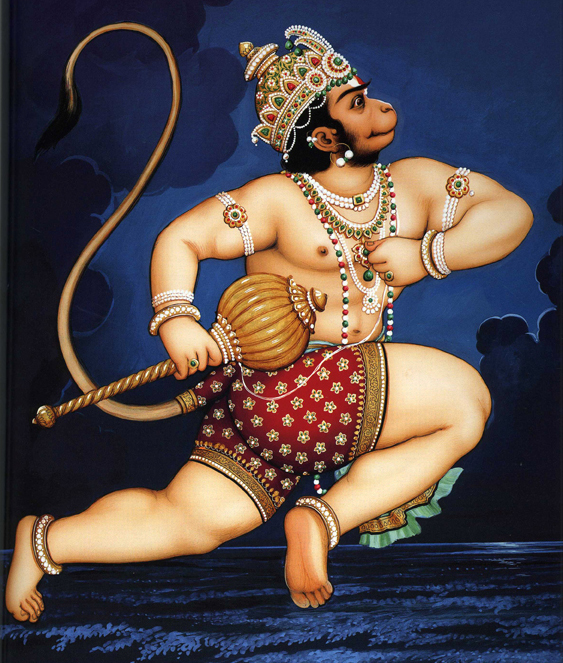
\includegraphics[width=100mm]{mahavirahanuman.jpg}}
\rput[lb](\mylengthone,42.5mm){\usebox\IBox}
\setlength{\mylengthone}{\coverinside + \coverwidth + \bookspine} 
\rput[lb](\mylengthone,32mm){\parbox{\coverwidth}{\centering\fontsize{18}{27}\selectfont\color{white}{व्याख्याकार}}}
\rput[lb](\mylengthone,20mm){\parbox{\coverwidth}{\centering\fontsize{22}{33}\selectfont\color{white}{\textbf{जगद्गुरु रामानन्दाचार्य स्वामी रामभद्राचार्य}}}}
%%%%%%%%%%%%%%%%%%%%%%%%%%%%%%%%%%%%%%%%%%%%%%%%%%
% THIS IS THE BOOK BACKCOVER
%%%%%%%%%%%%%%%%%%%%%%%%%%%%%%%%%%%%%%%%%%%%%%%%%%
\setlength{\mylengthone}{\coverinside + \covermargin} 
\setlength{\mylengthtwo}{\coverwidth - \covermargin*\real{2}} 
\rput[tl](\mylengthone,200.5mm){\parbox{\mylengthtwo}{\fontsize{13.5}{17}\selectfont\color{white} \begin{sloppypar}\justifying\hyphenrules{nohyphenation} पद्मविभूषण-विभूषित जगद्गुरु रामानन्दाचार्य \textbf{स्वामी रामभद्राचार्य} भारतके प्रख्यात विद्वान्, वैयाकरण, शिक्षाविद्, बहुभाषाविद्, महाकवि, भाष्यकार, दार्शनिक, रचनाकार, संगीतकार, प्रवचनकार, कथाकार, व धर्मगुरु हैं। वे चित्रकूट-स्थित \textbf{श्रीतुलसीपीठ}के संस्थापक एवं अध्यक्ष और \textbf{जगद्गुरु रामभद्राचार्य दिव्याङ्ग विश्वविद्यालय चित्रकूट}के संस्थापक एवं आजीवन कुलाधिपति हैं। स्वामी रामभद्राचार्य दो मासकी आयुसे प्रज्ञाचक्षु होते हुए भी २२~भाषाओंके ज्ञाता, अनेक भाषाओंमें आशुकवि, और शताधिक ग्रन्थोंके रचयिता हैं। उनकी रचनाओंमें चार महाकाव्य (दो संस्कृत और दो हिन्दीमें), रामचरितमानसपर हिन्दी टीका, अष्टाध्यायीपर गद्य और पद्यमें संस्कृत वृत्तियाँ, और प्रस्थानत्रयीपर (ब्रह्मसूत्र, भगवद्गीता, और प्रधान उपनिषदोंपर) संस्कृत और हिन्दी भाष्य प्रमुख हैं। वे तुलसीदासपर भारतके मूर्धन्य विशेषज्ञोंमें गिने जाते हैं और रामचरितमानसके एक प्रामाणिक संस्करणके संपादक हैं।\end{sloppypar}
\begin{sloppypar}\justifying\hyphenrules{nohyphenation} प्रस्तुत पुस्तक सनातन धर्मके सर्वाधिक लोकप्रिय स्तोत्र \textbf{श्रीहनुमान्‌-चालीसा}पर स्वामी रामभद्राचार्यकी \textbf{\textit{महावीरी}} व्याख्याका तृतीय संस्करण है। ईस्वी सन् १९८३में मात्र एक दिनमें प्रणीत इस व्याख्याको राम\-चरित\-मानसके अंग्रेज़ी व हिन्दी अनुवादक डॉ.~रामचन्द्र प्रसादने \textit{श्रीहनुमान्‌-चालीसा}की ‘सर्वश्रेष्ठ व्याख्या’ कहा है। अनेक टिप्पणियों और परिशिष्टों सहित \textit{महावीरी} व्याख्याका परिवर्धित अंग्रेज़ी अनुवाद भी {\engtextfont {\relscale{0.75} \textit{\textbf{Mahāvīrī}: Hanumān-Cālīsā Demystified}}} नामसे प्रकाशित हो चुका है।\end{sloppypar}}}
\newsavebox\separator
\sbox\separator{
\includegraphics[scale=1]{vectorianseparator01white.png}}
\rput[b](67.25mm,94mm){\usebox\separator}
% ISBN Barcode and logo
\rput[lb](83mm,39.75mm){\parbox{3cm}{\fontsize{11}{15}\selectfont\color{white}{\rupeefonttwo {\relscale{0.93} \textasciigrave}}\fontsize{10}{15}\selectfont\color{white}{\engtextfont 50}}}
\rput[rb](122.5mm,38.5mm){\parbox{3cm}{\fontsize{13.5}{15}\selectfont\color{white}\raggedleft विशिष्ट मूल्य}}
% Logo is between the lines x=88.5mm,y=15mm,x=128mm,y=38mm 
\rput[r](122.5mm,26.5mm){\colorbox{white}{\EANisbn[SC2]}}
% put the logo on the back cover
\setlength{\mylengthtwo}{\coverinside + \covermargin + 10mm} \newsavebox\logoboxcover
\sbox\logoboxcover{
\includegraphics[width=0.75in]{logo.png}}
\rput[lb](\mylengthone,\mylengthtwo){\usebox\logoboxcover}
% Publisher information
\setlength{\mylengthtwo}{\coverinside + \covermargin + 5mm} 
\rput[lb](\mylengthone,\mylengthtwo){\parbox{14cm}{\fontsize{14}{15.75}\selectfont\color{white}{\textbf{\ \ ज.रा.दि.वि.}}}}
\setlength{\mylengthtwo}{\coverinside + \covermargin} 
\rput[lb](\mylengthone,\mylengthtwo){\parbox{14cm}{\fontsize{10}{15}\selectfont\color{white}{\engtextfont www.jrhu.com}}}
%\psline[linecolor=white](15mm,0mm)(15mm,216mm)
%\psline[linecolor=white](0mm,15mm)(140mm,15mm)
\end{pspicture}
\end{document}
